\documentclass[11pt]{article}
\usepackage[a4paper, portrait, margin=1in]{geometry}
\usepackage{graphicx}
\usepackage{hyperref}
\usepackage{caption}
\usepackage[labelformat=simple]{subcaption}    %%Adding option to remove parenthesis
\renewcommand{\thesubfigure}{\normalsize Figure \thefigure. (\alph{subfigure}):}
% \usepackage{subcaption}
% \usepackage{subcaption}
%\usepackage{dirtytalk}
\usepackage{float}
\usepackage{eldar_report}
% Useful packages
\usepackage{amsmath}
% \newcommand\norm[1]{\lVert#1\rVert}
\newcommand\normx[1]{\Vert#1\Vert}
\usepackage{graphicx}
\usepackage{lifetime}
\newcommand{\Dana}[1]{\textcolor{purple}{\bf Dana: #1}}
\newcommand{\Tom}[1]{\textcolor{purple}{\bf Julian: #1}}


\begin{document}

\title{Robustness of Multi-Label Neural Networks}

\author{
    \textbf{Julian Mour} \\
    \\
    Advisor: Dana Drachsler Cohen\\
    Technion - Israel Institute of Technology
}

\maketitle

\section{Introduction}

In the last years, many works have demonstrated that deep neural networks (DNNs) are susceptible to a variety of adversarial example attacks, e.g.,~\cite{ref7,ref15,szegedy2014intriguing,ref17,ref29,ref56}. Most adversarial attacks add small changes to the input that fool the network. However, some attacks, known as $L_0$ attacks, focus on perturbing a very small number of pixels (e.g., one) to an arbitrary value~\cite{OnePixelAttack, alatalo2021chromatic, vargas2019understanding}. This type of attack is very effective for concealing adversarial modification in practice, and it can provide geometrical theoretical insight into the input space of a classifier. %Previous studies have shown that given an input image and a classifier (e.g. convolutional neural network), a perturbation of a single pixel or a very small and almost imperceptible perturbation of all pixels in the input image\cite{szegedy2014intriguing} can lead to misclassification. 
%Examining different approaches for adversarial attacks may help network designers gain a deeper understanding of the vulnerabilities of their networks and then utilize that information to improve the network's robustness.\Dana{a bit general}
These attacks are usually local: for each input, they perform a computation to determine the perturbation, which may take a few minutes. Furthermore, these attacks are not robust to input transformation, so each input must be processed differently.

In this thesis, we will design universal $L_0$ attacks, which rely on programs.
The key idea is that program can be specific to input but can be executed much faster and thus will be easier compared to prior attacks.
The program will determine which pixels to perturb and to which values. 
 %is to develop a framework for synthesizing universal adversarial programs. A program should, given an unknown input image, perturb a small number of pixels in order to carry out a successful untargeted attack. 
 Unlike previous adversarial attack methods, our programs do not employ independent optimization for each image but rather find structures/rules that can be applied to every new input to identify which pixels will be perturbed and how. 
 Our focus is on programs that have two stages. As the first stage, the goal is to limit the search space for a successful attack to a relatively small area in the input image. During the second stage, the focus is primarily on identifying the perturbation (its location and magnitude) within that small area.  
 %We concentrate on programs that have conditions that are based on different areas of the input in order to determine the perturbation. We also examine programs that use neural networks to determine the location and magnitude of the perturbation.
 
 Our key idea is to formulate this problem as an optimization problem in which we try to find the optimal program. Two methods have been considered in terms of the initial stage of the program. First is an evaluation search that is trained on a limited set of inputs and given a set of possible program instructions. With each successive iteration, the search seeks to improve the program based on previously generated programs. In the second technique, a deep neural network is used to predict the locations and magnitudes of the perturbed pixels. For the second stage of the program, we developed a small program that iteratively examined all possibilities in a specific area.  
 
 In our preliminary research, we implemented our optimization approach on CIFAR-10 dataset on ResNet-18~\cite{he2015deep} and evaluated it. We compared our results to the well-known "one-pixel attack method"~\cite{OnePixelAttack} which is our baseline. Our initial results indicate that our program generated attacks that had almost the same success rate as the baseline, but with much shorter execution times and significantly fewer queries.  

In the future, we intend to improve our algorithms to ensure a greater success rate of the attacks and shorter execution times with fewer queries. Additionally, we would like to leverage our programs to provide a better understanding of the network's decision boundaries and the factors that contribute to an attack's success.

\section{Problem Definition}
In this section, we define the problem we address. Informally, we are interested in synthesizing a program that, given a new image, unknown during the synthesizing process, can perturb a small number of pixels in order to perform a successful untargeted attack.

Formally, Given a classifier $N$, a set $X$ of $n$ test images and correspond true classes $c_1, c_2, ..., c_n$, our goal is to synthesis a universal perturbation program $P$ such that $N$ classified as many perturbed images ($P(x_i)$ s.t. $x_i\in X$) as possible to some label $t_i \neq c_i$. In order to ensure that the perturbation is relatively small when applied to natural image $x_i$ we add the constraint $||P(x_i)-x_i||_0\leq d$. In our case, we use $d={1, 2,..,5}$.

\begin{equation*}
\begin{array}{rrclcl}
\displaystyle \max_P & \multicolumn{2}{l}{\sum_{i=1}^n \mathbbm{1}_{class(N(P(x_i)))\neq c_i}}\\
\textrm{s.t.} & \forall x_i\in X,\quad||P(x_i)-x_i||_0\leq d
\end{array}
\end{equation*}


\section{Our Approach}

In this thesis, we will synthesize universal programs, that will generate successful universal adversarial $L_0$ attacks. For the first stage of the program, we consider two different approaches:
\begin{itemize}
    \item Evolution Search - The desired program will be based on the RGB values of pixels and small spatial regions within the image. The desired program will be created using evolution search optimization~\cite{GOLDBERG199169, real2019regularized}. In this program, a few learnable "filters" will be used to determine the location and the magnitude of the perturbation. Each filter consists of several learnable parameters including the spatial size ($1\times1$ or $3\times3$ or $5\times5$) of the filter, the channel (red, green or blue), its value boundaries, and the perturbation. Accordingly, our current settings determine whether a pixel is "agreed" on a specific filter if the mean value of the pixels in the selected channel in some spatial size around the pixel lies within the specified boundaries (higher/lower than some numeric threshold). A perturbation will be applied to pixels that "agree" with the greatest number of filters. Basically, the synthesized program $P$ is a set of filters $F$ that takes a "natural" input image $x_i$ and calculates the magnitudes and positions of the perturbations outputs them. 
    \item Deep Learning - By using this approach, we will build a CNN that will take an image as an input, determine the position (regression task) and the magnitude of the perturbation (classification task - each class represents a possible perturbation) as an output. The network will be trained using individual attacks on the trainset. 
\end{itemize}
There are several differences between the two approaches mentioned above. Synthesized by evolution search programs may be more straightforward and interpretable than deep learning techniques. Moreover, evolution search does not require the creation of a new dataset of successful adversarial attacks. On the other hand, the deep learning approach is based on a CNN which is regarded as a strong model for identifying features in images.

During the second stage of the program, after calculating the suggested perturbation (location and magnitude) in the first stage, the program will attempt to locate an attack within the same spatial area as the suggested perturbation. The current implementation involves systematically searching around the suggested area in successive iterations, each time trying to go further from the suggested pixel.


\section{Preliminary Results}
We implemented our approach and evaluated it on the CIFAR-10 test dataset (consisting of images from ten classes) and ResNet-18 as the "attacked" network. We will calculate the success rate of the attacks which generated by our program to determine whether it is successful. Success rate is the percentage of the successful attacks among originally correctly classified images:
\begin{equation*}
\text{Success Rate}= \frac{\sum_{i=1}^n \mathbbm{1}_{class(N(P(x_i)))\neq c_i \land class(N(x_i))= c_i}}{\sum_{i=1}^n \mathbbm{1}_{class(N(x_i))=c_i}} \cdot 100
\end{equation*}
Where $n=10,000$ is number of test images, $N$ is the classification CNN, $P$ is the synthesized program, and $x_i$ is an image from class $c_i$.

Using the current implementation, we achieved a success rate of 22.28\% on ResNet-18 when on average each successful attack (on one image) takes 0.07 seconds and 34.32 queries. The program was restricted to only perturb one pixel per image, and to only one possible perturbation (maximum values of the three channels). We evaluated that the maximum possible success rate with our current setting (one possible perturbation of one pixel) is 24.81\% when we use brute force (iterating over all possible pixels) which gives the optimal solution but is very inefficient in terms of execution time and the number of queries. Furthermore we evaluated the well-known "one-pixel attack" method~\cite{OnePixelAttack} on the current setting. We have achieved a success rate of 23.96\% using that attack, with an average execution time of 0.45 seconds and an average of 232.59 queries - both calculated per one input image and only for successful attacks. Figure \ref{fig:results} shows the comparison between the results of our method to the results of the "one pixel attack" method. 

\begin{figure}
     \centering
     \begin{subfigure}[b]{0.4\textwidth}
         \centering
         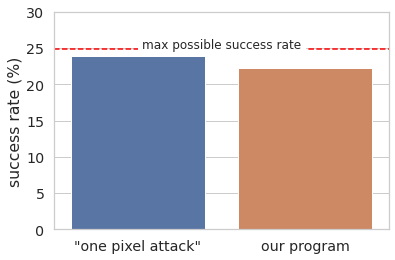
\includegraphics[width=\textwidth]{success_rate.png}
         \caption{Success Rate}
         \label{Success Rate}
     \end{subfigure}
     \hfill
     \begin{subfigure}[b]{0.4\textwidth}
         \centering
         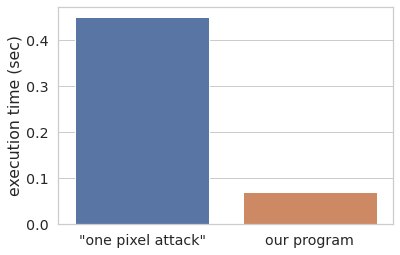
\includegraphics[width=\textwidth]{execution_time.png}
         \caption{Average Execution Times}
         \label{execution time}
     \end{subfigure}
     \hfill
     \begin{subfigure}[b]{0.4\textwidth}
         \centering
         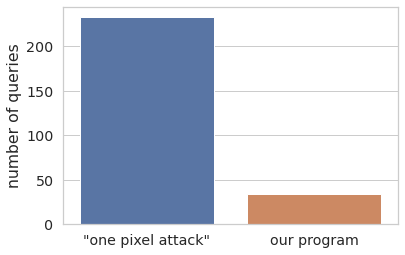
\includegraphics[width=\textwidth]{number_queries.png}
         \caption{Average Number of Queries}
         \label{number queries}
     \end{subfigure}
        \caption{Comparison between the results of our method to the results of the "one pixel attack" method.}
        \label{fig:results}
\end{figure}

\section{Future Research Objectives}
In light of the preliminary work, we aim to further explore our ideas in the following directions:
\begin{itemize}
    \item Improved algorithm: success rate, execution times and number of queries - As a result of the current implementations and settings of our two approaches, the success rate of the attacks generated by the program is lower than our baseline. Therefore, we will implement different evolution methods, take a different approach to program instruction design, and develop a different architecture (e.g. transformers~\cite{vaswani2017attention}) for the deep network approach in order to increase success rates. While improving the success rate, we will strive to keep execution times as short as possible with a low number of queries.
    \item Explainability - One possible advantage of using a universal program to generate adversarial examples is to be able to explain the network's decision boundaries and the reasons that lead to the success of attacks. As an example, by synthesizing a program, we can determine which spatial regions or channels are relevant to the success of the attack. Using the deep learning approach, we are able to use other known tools for an explanation, such as LIME~\cite{ribeiro2016why}.
\end{itemize}

\section{Related Work}
Our thesis lies at the intersection of adversarial attacks and program synthesis. We next review some
related work.
\subsection{Adversarial Attacks}
Several aspects can be used to classify adversarial attacks~\cite{taxonomy}:
\begin{itemize}
    \item Targeted Vs. Untargeted - A targeted attack~\cite{papernot2015limitations} attempts to mislead a classifier by classifying input to a \textit{specific class} that differs from the true class of input. In untargeted attacks~\cite{ref7}, the goal is to cause the classifier to classify the input to \textit{any class} that is different from the true class.
    \item Individual Vs. Universal - Individual attacks generate different attacks for each different input, by optimizing the attack based on the input~\cite{ref7,papernot2015limitations,moosavidezfooli2016deepfool}. Universal attacks, on the other hand, generate one attack for all possible inputs. Studies from the last few years have indicated that universal adversarial attacks are capable of generalizing well to unseen data. The first method for universal adversarial attack was based on accumulating perturbations iteratively by composing perturbations for each data point~\cite{moosavidezfooli2017universal}. Other studies have used singular vectors~\cite{khrulkov2017art} and networks for adversary generation (NAGs)~\cite{mopuri2018nag}.
    \item White box Vs. Black box - In white box attacks, the architecture, weights, and parameters of the model are known to the adversary. First, white box adversarial attacks were derived through the generation of artificial perturbations using gradient-based optimization~\cite{szegedy2014intriguing}. There have been numerous works since then that have demonstrated different approaches to generating white-box adversarial attacks, such as FGSM\cite{ref7}, JSMA~\cite{papernot2015limitations}, and Deepfool~\cite{moosavidezfooli2016deepfool}. Attackers using black box methods assume they can only query the model without any further knowledge of it. Several studies have shown that a black-box approach can lead to generating successful attacks~\cite{BlackBox1, BlackBox2, BlackBox3, BlackBox4}.
\end{itemize}

Additionally, we investigate $L_0$ attacks, which aim to modify a small number of pixels. In previous studies, it has been demonstrated that even a single pixel perturbation can lead to successful attacks\cite{OnePixelAttack, alatalo2021chromatic, vargas2019understanding}.

\subsection{Program synthesis}
Program synthesis is the task of automatically generating a computer program from user requirements. It has been studied for decades and shown success in a variety of fields,
such as data wrangling\cite{inbook}, code repair\cite{d39antoni2016qlose}, code suggestions\cite{10.1145/2594291.2594321}, probabilistic modeling\cite{nori2015efficient} and superoptimization\cite{10.1145/36206.36194}. Later, constructive techniques have been developed, such as enumerative
search\cite{6679385}, programming by examples\cite{inbook}, constraint solving\cite{CSP}, stochastic search\cite{schkufza2012stochastic}, neural program synthesis\cite{parisotto2016neurosymbolic} and genetic programming\cite{Koza92}. In our preliminary
work, we focused on a variant of genetic search.



\bibliography{bibliography}
\bibliographystyle{plain}

\end{document}
